\label{chap:pfp}
  \section*{History of Changes}

  {\bfseries 2011-12-19} Initial revision.

  {\bfseries 2012-01-04} Listed briefly the signal connections between front
  panel and processor boards.

  {\bfseries 2012-01-09} Added revision B schematics, bill of materials and parts index.

  {\bfseries 2012-01-15} Minor modifications to the schematics and matching
  description. Added discussion on configuring and tuning the front
  panel.

  {\bfseries 2012-01-18} Added front panel controller and started section of the
  front panel's theory of operation.

  {\bfseries 2012-01-20} Added theory of operation of sequencer and system device and
  updated rendered images of boards, schematics and bills of materials.

\section{Introduction}

The CFT minicomputer is intended to be similar to a 1960s
minicomputer, and it could never be similar enough without a
programmer's front panel.

The front panel is serves two purposes: to inspect the state of the
computer, and to modify the state of the computer. State inspection is
made possible via a number of lights corresponding to the binary state
of most of the computer's crucial signals. State modification is via a
number of switches which control the operation of the computer's main
units and provide user input.

The CFT front panel is expected to provide a number of services.

\begin{itemize}
\item During construction, it will provide a means of testing most of
  the computer's individual units on their own. With some rewiring or
  reconfiguration, all of the computer's features can be tested.

\item After construction, it will allow microcode to be inspected and
  thereby debugged.

\item It will also allow the computer to be programmed without a
  ROM. A front panel was usually the only built-in means of
  programming a minicomputer, and in many cases was the only way the
  computer could be booted up.

\item It will allow debugging of software and hardware by allowing the
  computer to be stopped, its state inspected and perhaps changed, and
  then resuming execution.

\item Finally, it will allow the state of the running computer to be
  inspected with varying degrees of success.\footnote{The human eye
    is, of course, incapable of registering light pulses with MHz
    frequencies, but the panel lights register these with varying
    intensities of light.}

\end{itemize}

\section{Layout of the Front Panel}

\begin{figure}[t]
\centering
\includegraphics[width=0.8\textwidth]{../../panel/front-panel-v2-small.jpg}\\
\caption{\label{fig-panel}A first draft of the CFT front panel.}
\end{figure}

The CFT minicomputer is intended to be built into a 19-inch rack-mount case, 6U
in height, making it approximately 19" by 10.5" (482.6mm by 266.7mm) in size.

The panel displays the state of the computer on 118 console lights. For lower
consumption, convenience and longevity, these are light-emitting diodes (LEDs).

30 toggle switches allow the computer's state to be modified, and user input to
be provided.

Computer power and panel locking is controlled by a three-position key switch.

All lights and switches are displaying multi-bit quantities are arranged with
the most significant bit to the right, in the conventional notation of binary
numbers. Bit numbers start at 0, which is the least significant bit or
rightmost light. This follows the conventional notation of powers-of-two.

\subsection{Console Lights}

The console lights are arranged in six rows.

\subsubsection{Memory Controller}

The leftmost bank of lights on the top row displays the status of the banking
memory controller, if it is installed.

If banking has been enabled, a green light marked \lt{ENABLED} indicates
this. Eight yellow lights marked \lt{AEXT7}–\lt{AEXT0} indicate the bank
currently selected.

Conventionally, the memory controller addresses up to one MWord of ROM mapped
in the top MWord of the 21-bit address space (physical addresses
\hex{20:0000}–\hex{3F:FFFF}). Thus, light \lt{AEXT7} also indicates that a ROM
bank may be selected (this depends on the particular configuration of the
memory board or boards: please refer to~\ccf{chap:mem} for detailed
information). The light is thus marked \lt{AEXT7/ROM}).

If the memory controller board is not installed, these lights remain off.

\subsubsection{Interrupt Controller}

The middle bank of lights on the top row indicates the status of the optional
interrupt controller on eight lights marked \lt{INT7}–\lt{INT0}.

Each of these lights will indicate a number of different conditions depending
on its colour.

\begin{itemize}
  \item {\bfseries Off}: the computer is ignoring this interrupt line, and there is
    no interrupt activity.
  \item {\bfseries Green}: the interrupt line is being used by the computer, but
    there is no interrupt activity.
  \item {\bfseries Orange}: the interrupt line is being used by
    the computer, with interrupt activity.
  \item {\bfseries Red}: there is interrupt activity, but it is being ignored
    by the computer.
\end{itemize}

Because interrupt pulses are too short and relatively rare, in order to make
them visible to the naked eye, each interrupt pulse will illuminate the light
red or orange for approximately one tenth of a second.

\subsubsection{Miscellaneous Lights}

Three green lights marked \lt{GEN2}–\lt{GEN0} are located at the right of the
topmost row. These are reserved for generic use. Hardware may indicate its
status on any of them via physical two-wire connections.

\subsubsection{State}

The leftmost bank of lights on the second row from the top indicates the
processor's major operating states.

\begin{itemize}
\item \lt{RUN} (green) indicates the processor clock is running.
\item \lt{STOP} (red) when the \lt{RUN} light is off and this light is
  on, the processor clock is stopped and the front panel switches are
  active (provided the front panel is unlocked). When the \lt{RUN}
  light is on and this light flashes briefly, some device is
  introducing wait states by briefly halting the processor.
\item \lt{FETCH} (yellow) indicates the processor is in the Fetch state,
  retrieving its next instruction from memory.
\item \lt{EXEC} (yellow) indicates the processor is in the Execute state,
  performing the task identified by the previously retrieved instruction.
\item \lt{INT} (yellow) indicates the processor is handling a previously
  retrieved interrupt. Because interrupt states are too short and relatively
  rare, in order to make them visible to the naked eye, each interrupt pulse
  will illuminate this light for approximately one tenth of a second.
\end{itemize}

\subsubsection{Program Counter}

Sixteen red lights on the second row from the top indicate the current value of
the \PC. When the \lt{FETCH} light is illuminated, the \PC{} contains the
address in memory of the instructing being fetched. When the \lt{EXEC} light is
illuminated, the \PC{} indicates the address of the {\em next\/} instruction to
be executed (as long as no branching takes place in the current instruction).

\subsubsection{Flags}

Five green lights indicate the state of the five minor registers (flags) of the
processor.

\begin{itemize}
\item \lt{N} indicates bit 15 of the \A{} is set.
\item \lt{Z} indicates the \A{} is zero.
\item \lt{V} indicates an arithmetic overflow has been detected by the \ALU.
\item \lt{I} indicates that the processor allows interrupts.
\item \lt{L} indicates the state of the \Lreg{} register.
\end{itemize}

\subsubsection{Accumulator}

Immediately to the right of the \lt{L} light, on the second row from the top,
are 16 red lights representing the current value of the \A{} register. The
placement is such that the $(L,A)$ pair is easy to inspect when adding or
rotating.

\subsubsection{Multi-Function Display}

The Multi-Function Display occupies the third row of lights. Using a switch,
the user may choose to display the value of the Front Panel Output Register,
the Data Register (\DR), and the current micro-Address vector. In the latter
case, the meanings of each bit are marked below each light. The most
significant bit is not used in this case.

\subsubsection{Memory}

The status of the memory and I/O sequencing is shown on a bank of four lights,
on the fourth row from the top (second row from the bottom). The meanings of
these lights are as follows:

\begin{itemize}
\item \lt{MEM} (yellow) indicates memory space is being accessed.
\item \lt{IO} (yellow) indicates Input/Output space is being accessed.
\item \lt{R} (green) indicates a read cycle is in progress.
\item \lt{W} (red) indicates a write cycle is in progress.
\end{itemize}

These lights are pairwise mutually exclusive. The four combinations of them
describe the nature of the memory or I/O access (memory read, memory write, I/O
read, I/O write). Please note that these lights are, in essence, part of the
micro-instruction as described below.

\subsubsection{Instruction Register}

The contents of the \IR{} are displayed to the right of the memory lights. The
instruction fields (operation, I, R, and operand field) are indicated below the
lights. Alternating yellow and red lights are used for each field to aid
reading the IR.

Please note that the \lt{L} light indicates {\em exactly\/} the corresponding
field in an instruction: register mode is active when the light is {\em off}.

\subsubsection{Micro-Instruction}

The bottom row of lights indicates most of the control signals emanating from
the Microcode ROM (the memory control signals, described above, are the only
exception). These are useful in debugging the machine at the microcode level.

\subsection{Switches}

There are 30 switches and a key switch arranged in two rows below the
bottom-most row of lights. The top row is the Switch Register (16
switches), while the 

\subsubsection{Key Lock}

The key lock operates computer power and controls access to the front
panel.

Computer power is off with the key in the \sw{OFF} position.

Computer power is on with the key in the \sw{ON} position. In this position,
most panel switches are locked. These are the exceptions:

\begin{itemize}
\item The key switch may be operated.
\item The 16 Switch Register switches may be used to register 16-bit values
  read by the computer via the Front Panel System Device.
\item The \sw{VERBOSE}/\sw{TERSE} switch may be operated to enable or disable
  some front panel lights.
\item The Multi-Function Display Selector may be operated to change what is
  displayed on the Multi-Function Display.
\end{itemize}

With the key switch in the \sw{PANEL} position, all panel switches are unlocked
and enabled.

\subsubsection{Switch Register}

The switch register comprises 16 toggle switches located below the bottom-most
row of lights. These may be used to provide instructions or values to be stored
in processor registers when the computer is halted, or read directly by
computer programs via the Front Panel System Device when the computer is
running. This is the only form of user input of the unexpanded computer.

The switches are aligned with the corresponding bits of the various red
register lights and numbered in the same power-of-two convention as register
display lights. Switches are grouped in four four-bit groups for easier
reading.

Push a switch up to set the corresponding bit. Push it down to clear it.

\subsubsection{Run Control}

The Run Control switch group is located on the bottom row of switches,
below the Switch Register switches. It comprises three momentary
action switches with six functions. Switches may be pushed up or down
momentarily to activate their corresponding functions. These are:

\begin{description}
\item{\bfseries\sw{RESET}} Push the leftmost switch up to reset the
computer.
\item{\bfseries\sw{START}} Push the leftmost switch down to reset the
computer and start the processor clock.
\item{\bfseries\sw{RUN}} Push the middle switch up to enable the computer
  clock and allow the computer to continue executing.
\item{\bfseries\sw{STOP}} Push the middle switch down to disable the
  computer clock. This halts the computer and activates the controls
  of the front panel. Please note that the clock is halted
  immediately, possibly in the middle of executing a
  microprogram. Examine the \lt{FETCH}, \lt{EXEC} and
  \lt{μADDR3}–\lt{μADDR0} lights to determine exactly where the
  machine stopped.
\item{\bfseries\sw{uSTEP}} Push the rightmost switch up to trigger a single
  clock pulse, advancing to the next microinstruction.
\item{\bfseries\sw{STEP}} Push the rightmost switch down to advance to the
  first execution clock of the next instruction. The computer's clock
  is briefly enabled until the end of the first fetch cycle
  encountered after the activation of the switch, and immediately
  halted. At that point, the Instruction Register will display the
  instruction about to be executed and the Program Counter will
  display the address of the {\em next\/} instruction to be executed
  (barring jumps or skips). An optional auto-repeat mechanism allows
  the computer to step over multiple instructions while the \sw{STEP}
  switch is depressed. To activate the auto-repeat, press and hold the
  switch. A single step will be performed. Approximately two seconds
  after, and approximately every second after that, further step
  operations will be performed.
\end{description}

\subsubsection{State modification}

The state modification group resides centred below the switch
register. It comprises seven momentary action action switches and one
on-on toggle switch performing 15 actions:

\begin{description}
\item{\bfseries\sw{LOAD ADDR}} Operate the leftmost switch up or down to load the
  contents of the Switch Register into the Program Counter.
\item{\bfseries\sw{LOAD IR}} Push the second switch up to load the contents
  of the Switch Register into the Instruction Register.
\item{\bfseries\sw{LOAD AC}} Push the second switch up to load the contents
  of the Switch Register into the \gls{Accumulator}.
\item{\bfseries\sw{MEMORY DEPOSIT}} Push the third switch up to store the
  contents of the Switch Register onto the memory address displayed in
  the address (Program Counter) bank of lights.
\item{\bfseries\sw{MEMORY DEP NEXT}} Push the third switch down to store the
  contents of the Switch Register onto the memory address displayed in
  the address (Program Counter) bank of lights. The Program Counter
  address is incremented by one after this. Repeated activations of
  this switch can fill a region of memory with the value of the Switch
  Register.
\item{\bfseries\sw{MEMORY EXAMINE}} Push the fourth switch up to load a
  value from memory into the \gls{Accumulator}. The memory address used is
  that of the Program Counter (address) lights.
\item{\bfseries\sw{MEMORY EXAM NEXT}} Push the fourth switch down to load a
  value from memory, and increment the Program Counter by
  one. Repeated activations of this switch allow regions of memory to
  be examined one word at a time.
\item{\bfseries\sw{INPUT/OUTPUT DEPOSIT}} Push the fifth switch up to
  perform the same function as the \sw{MEMORY DEPOSIT} switch, but for
  I/O space.
\item{\bfseries\sw{INPUT/OUTPUT DEP NEXT}} Push the fifth switch down to
  perform the same function as the \sw{MEMORY DEP NEXT} switch, but
  for I/O space.
\item{\bfseries\sw{INPUT/OUTPUT EXAMINE}} Push the sixth switch up to
  perform the same function as the \sw{MEMORY EXAMINE} switch, but for
  I/O space.
\item{\bfseries\sw{INPUT/OUTPUT EXAM NEXT}} Push the sixth switch down to
  perform the same function as the \sw{MEMORY EXAM NEXT} switch, but
  for I/O space.

\item{\bfseries\sw{RAM BNK}} The seventh switch is an on-on toggle switch,
  not a momentary action switch. When in the upper (\sw {RAM BNK})
  position, it maps 32 kWords of RAM to the top of the CFT address
  space. This is useful when the computer must be booted from the
  control panel. This setting is only valid while the \lt{ENABLED}
  light of the Memory Controller group is extinguished. Once the
  computer activates banking, the mapping is under its control and the
  position of this switch is ignored.
\item{\bfseries\sw{ROM BNK}} Likewise, when the switch is in the \sw{ROM
  BNK} position, 32 kWords of ROM are mapped to the top of the CFT
  address space. This position is required to execute the ROM
  bootstrap code directly after starting the machine.

\item{\bfseries\sw{IFR1}} Push the eighth switch up to send an interrupt 1
  (relatively high priority) pulse to the interrupt controller. This
  is used to provide asynchronous input to the computer, as long as
  the monitor software is aware of it.
\item{\bfseries\sw{IFR6}} Likewise, push the eighth switch down to send an
  interrupt 6 (relatively low priority) pulse to the interrupt
  controller.

\end{description}

All of the above functions, including the {\sw{RAM BNK}/\sw{ROM BNK}}
switch but {\em excluding\/} the \sw{IFR1}/\sw{IFR6} switch, are
locked out unless the key switch is in the \sw{PANEL} position, and
the clock is halted (\lt{RUN} light off; \lt{STOP} light on).

\subsubsection{Convenience and Panel Control Switches}

The rightmost group provides convenience functions:

\begin{description}
\item{\bfseries\sw{FAST}/\sw{SLOW}/\sw{TEST}} This three position toggle
  switch controls the speed of the system clock. In the \sw{FAST}
  position, the clock runs at its nominal speed. In the \sw{SLOW}
  position, the processor executes at a significantly increased clock
  period, in the order of one microsecond\footnote{The exact clock
    speed depends on the system clock and an internally configured
    clock divider.}). This executes approximately 1,000 clock ticks a
  second, or (very approximately) 100 instructions per second, making
  instructions visible on the panel lights. In the \sw{TEST} position,
  the clock period is increased even further, so that
  microinstructions become visible and approximately 10 instructions
  per second are executed. This is intended to allow testing
  microcode. In order to avoid potential glitches that would
  destabilise the system, the setting of this switch is ignored if the
  system is running or if front panel is locked via the key switch.

\item{\bfseries\sw{VERBOSE}/\sw{TERSE}} In the upper position, this switch
  enables all front panel lights for full diagnostics. In the interest
  of reducing light pollution and visual overloading, the lower
  position (\sw{TERSE}) disables a number of lights:
\begin{itemize}
\item The Memory Controller group,
\item The Interrupt Controller Controller group,
\item The Instruction Register,
\item The Flag Display,
\item The Memory Display, and
\item The μ-Instruction Display.
\end{itemize}

Some of these displays may be excluded from terse mode using jumpers
on the LED board. A mock-up of the panel in \sw{TERSE} mode is
available as~\fcf{fig-panel-terse}. Please note that the terms
‘verbose’ and ‘terse’ are under review.

\item{\bfseries Multi-Function Display Selector Switch} The rightmost switch
  on the bottom row of the front panel selects what is displayed on
  the Multi-Function Display bank. There are three options:
  \begin{description}
  \item{\bfseries\sw{OUTPUT REG}} Displays the contents of the Output Register
    on the Multi-Function Display. This register is provided by the
    Front Panel System Device and may be written to
    programmatically. It is the main form of user output available to
    an unexpanded CFT computer. On an expanded computer, the monitor
    program may use this register to display its high-level state,
    error codes, et cetera.
  \item{\bfseries\sw{DR}} Displays the Data Register on the Multi-Function
    Display.
  \item{\bfseries\sw{uADDR VEC}} Displays the 15-bit microcode address
    vector on the Multi-Function Display. The vector is made up of a
    number of components (conditions), each of which is marked under
    the corresponding light of the Multi-Function Display. This
    setting is intended to allow microcode testing.
  \end{description}
\end{description}

\begin{figure}
\centering
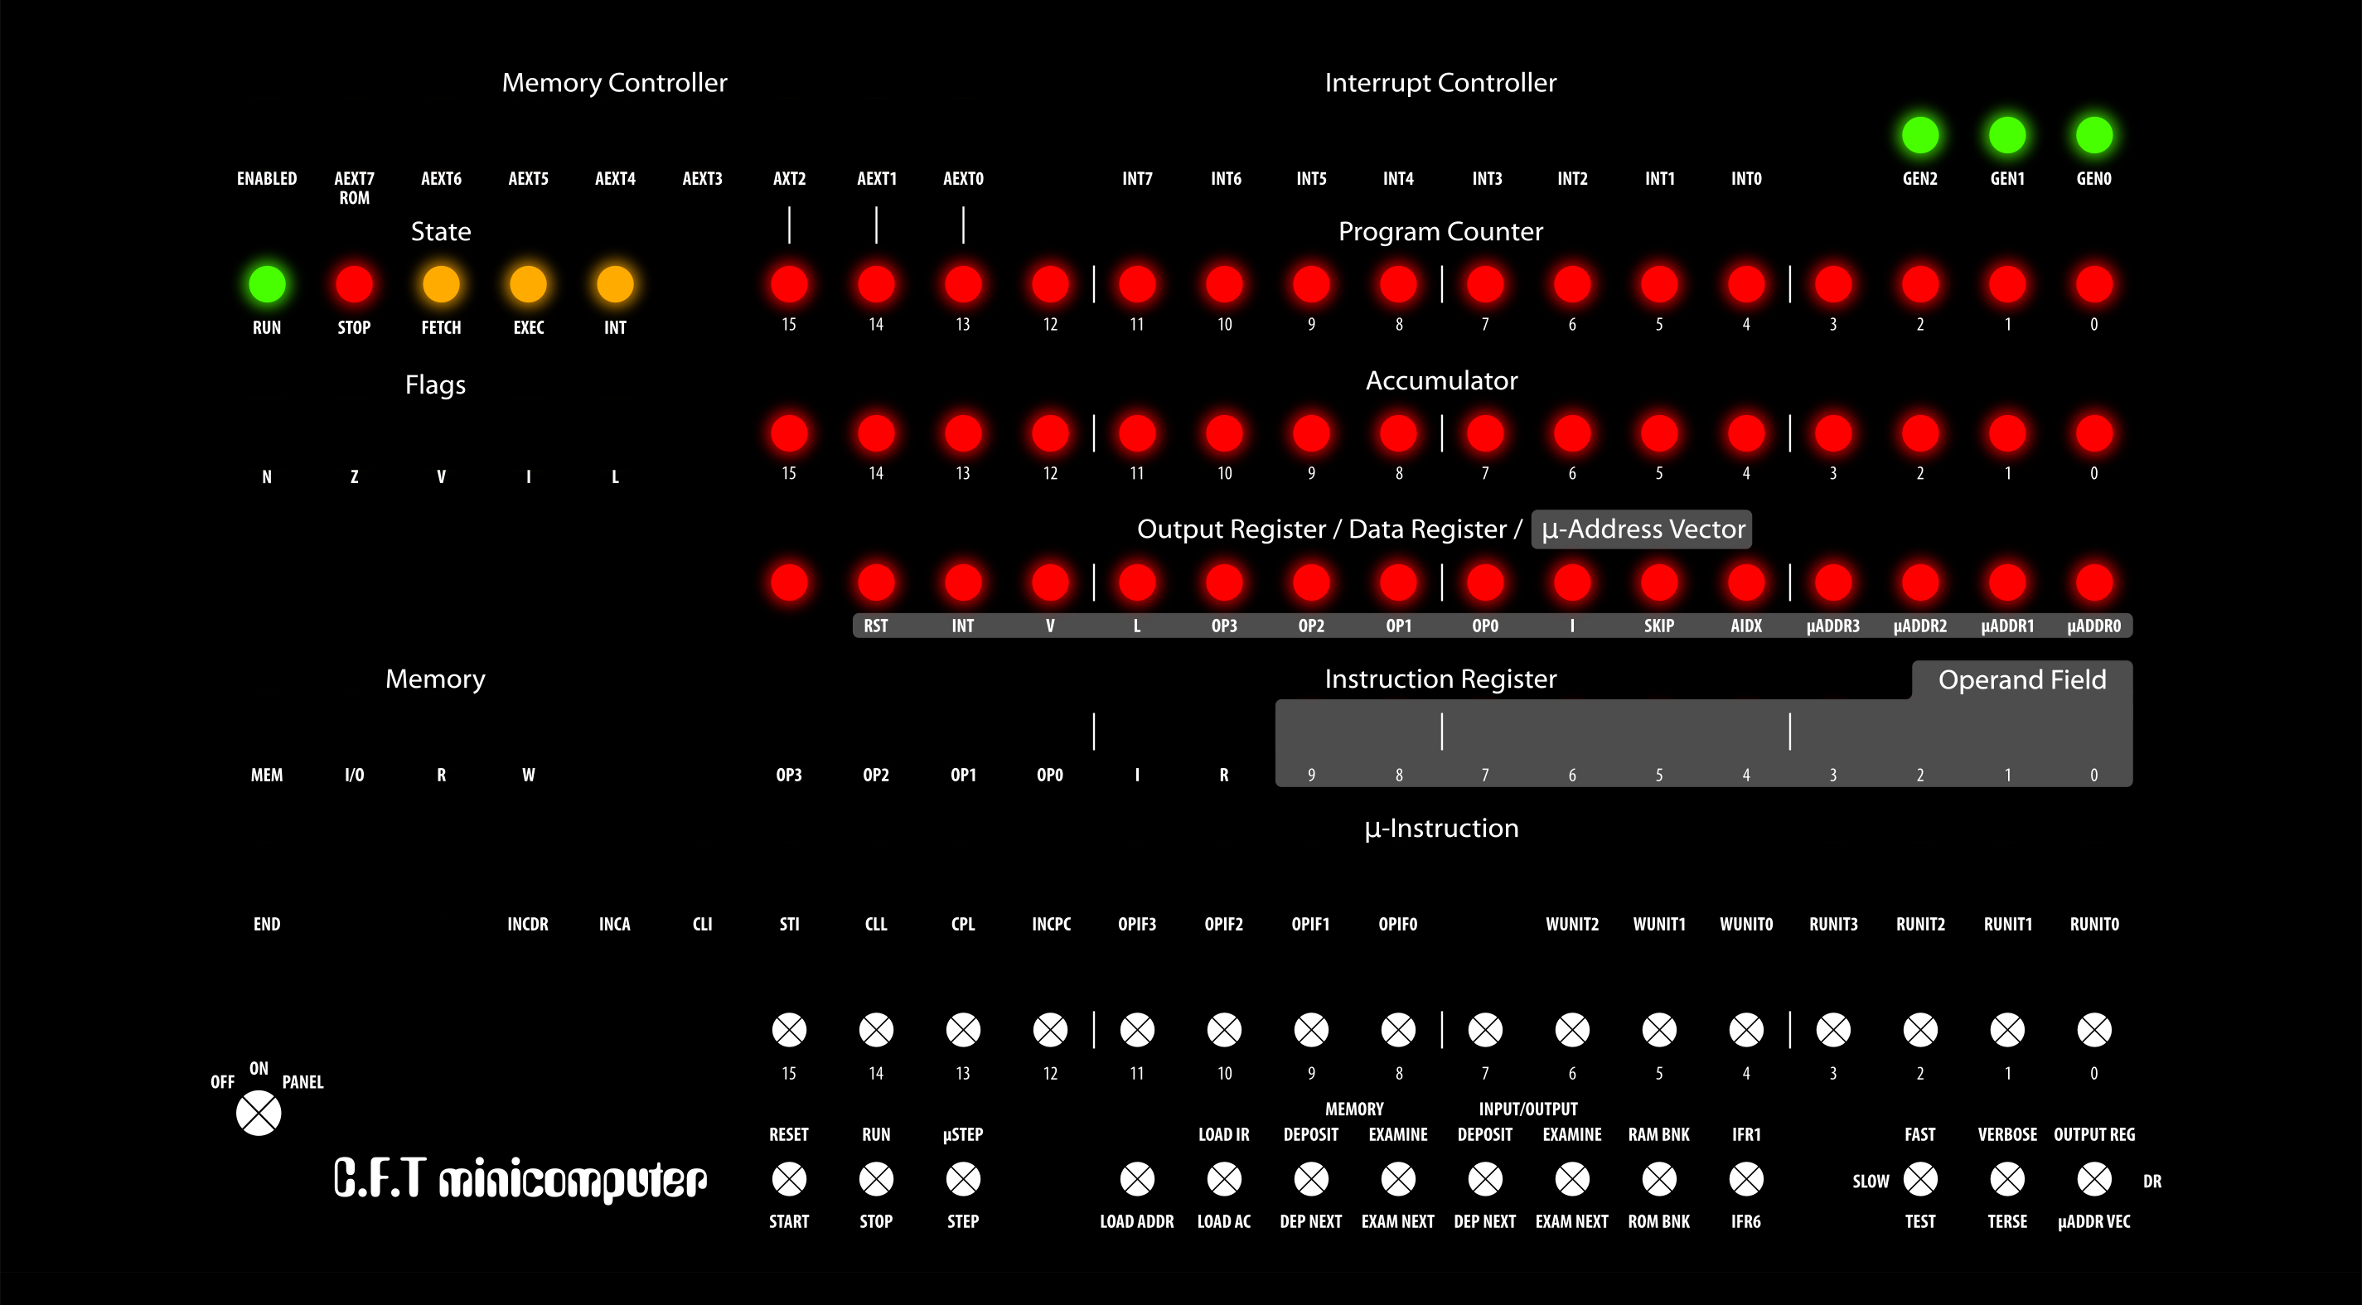
\includegraphics[width=0.8\columnwidth]{figs/front-panel-v2-terse-small.jpg}\\
\caption{\label{fig-panel-terse}A mock-up of the front panel running in \sw{TERSE} mode.}
\end{figure}

\subsection{Power}

A key switch at the lower right controls power. At the leftmost position, the
computer is off. When the key is turned one position to the right, the computer
is activated with most panel switches locked. With the key int he rightmost
position, all panel switches are unlocked and the panel may be used in its
entirety.

\section{Using the Front Panel}

This section describes how to use the computer via the front panel.

\subsection{Power}

Insert the key in the key switch. Turn the key to the \sw{PANEL}
position. The computer activates, performs power supply diagnostics,
goes through a reset cycle, and halts itself. The \lt{STOP} light
should illuminate at this point, and the Program Counter will indicate
a binary address of \bin{1111·1111·1111·0000}, or \hex{FFF0}.

\subsection{Boot from ROM}

With the computer freshly powered up and halted, or halted and reset,
move the \sw{ROM BNK}/\sw{RAM BNK} switch to the \sw{ROM BNK}
position.

Depress the \sw{RUN} or \sw{START} switch.

The computer boots from ROM address \hex{FFF0} and begins execution.

You may now secure the front panel by turning the key switch to the
\sw{ON} position.

\subsection{Toggle in Boot Code}

Ensure the computer is freshly powered up and halted, or halted and reset.

Set the Switch Register for a low value such as \bin{0000·0100·0000·0000}
(1kWord from start of memory). Depress \sw{SET ADDR}.

Set the Switch Register for the first value of the bootstrap
code. Depress \sw{MEMORY DEP NEXT}. Repeat as required.

Reset the Switch Register for the initial address of the bootstrap
program. Depress \sw{SET ADDR}.

Depress \sw{RUN}. The computer starts execution of the code from the
specified address.

You may now secure the front panel by turning the key switch to the
\sw{ON} position.

\subsection{Halting the Computer Forcibly}

With the key switch in the \sw{PANEL} position, depress \sw{STOP}. The
computer halts.

\subsection{Resetting the Computer}

With the key switch in the \sw{PANEL} position, depress \sw{RESET} or
\sw{START}. The computer resets. If the computer is running, ROM must
be fitted and the \sw{ROM BNK}/\sw{RAM BNK} switch must be in the
\sw{ROM BNK} position.

\subsection{Debugging with the Front Panel}

The front panel may be used to interrupt normal computer operation and
inspect or modify its state for debugging purposes. The computer can
then resume operation. The user should, however, be aware of a number
of considerations when using the front panel to do this:

\begin{itemize}
\item Operating the \sw{STOP} switch halts the computer
  mid-instruction. With a microprogram in execution, registers and
  control units may change. If necessary, the \sw{uSTEP} switch should
  be operated to complete the microprogram, that is until the
  \lt{FETCH} light illuminates. After which, if desired, the
  \sw{uSTEP} switch may be operated repeatedly until the \lt{EXECUTE}
  light illuminates, at which point an instruction has just been
  fetched and is about to be executed. It is safe to use the front
  panel for macro-debugging at this point.
\item Using the \sw{SET ADDR} switch modifies the \PC. When the
  computer resumes operation, this will effectively jump to the
  address set via the front panel. If this is not desired, the user
  must note the value of the \PC and manually restore it before
  continuing.
\item Using the memory and I/O functions also cause the \MAR{} to
  change. This is safe to do when using the \sw{STEP} switch, but not
  mid-microprogram.
\item Obviously, modifying the \IR{}, memory or I/O devices can have
  side effects on the running of the computer, but this is a desired
  feature of any control panel.
\end{itemize}

\section{Hardware Description}

\begin{figure*}
\centering
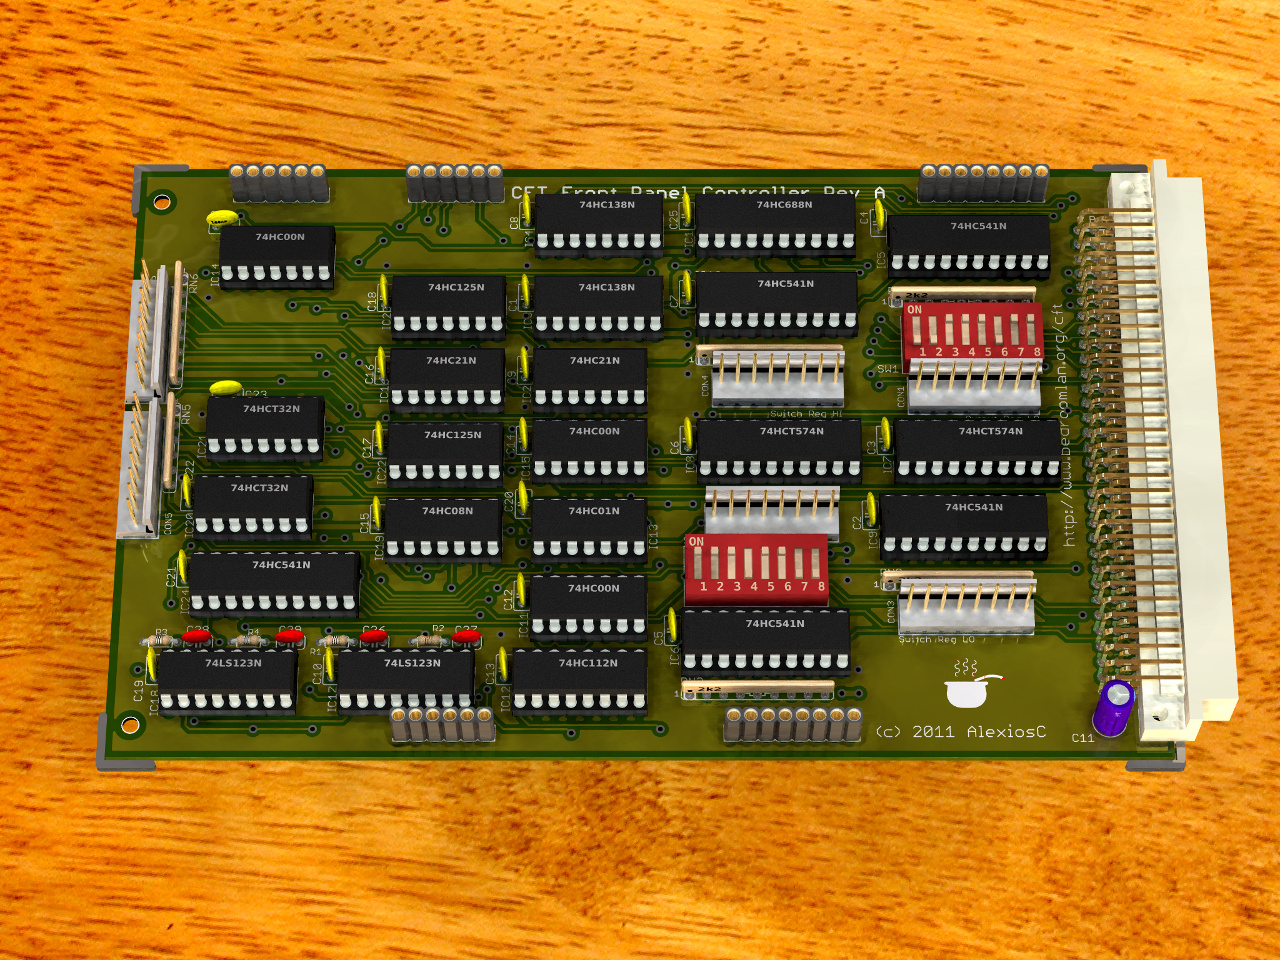
\includegraphics[width=0.8\textwidth]{figs/front-panel-controller-dip.jpg}\\
\caption[Rendered view of an assembled Front Panel
  Controller board]{\label{fig-rendered-fpc-dip}Rendered view of an assembled Front Panel
  Controller board. This is the original, \abbr{DIP} attempt and is shown here for
  historical reasons.}
\end{figure*}

\begin{figure*}
\centering
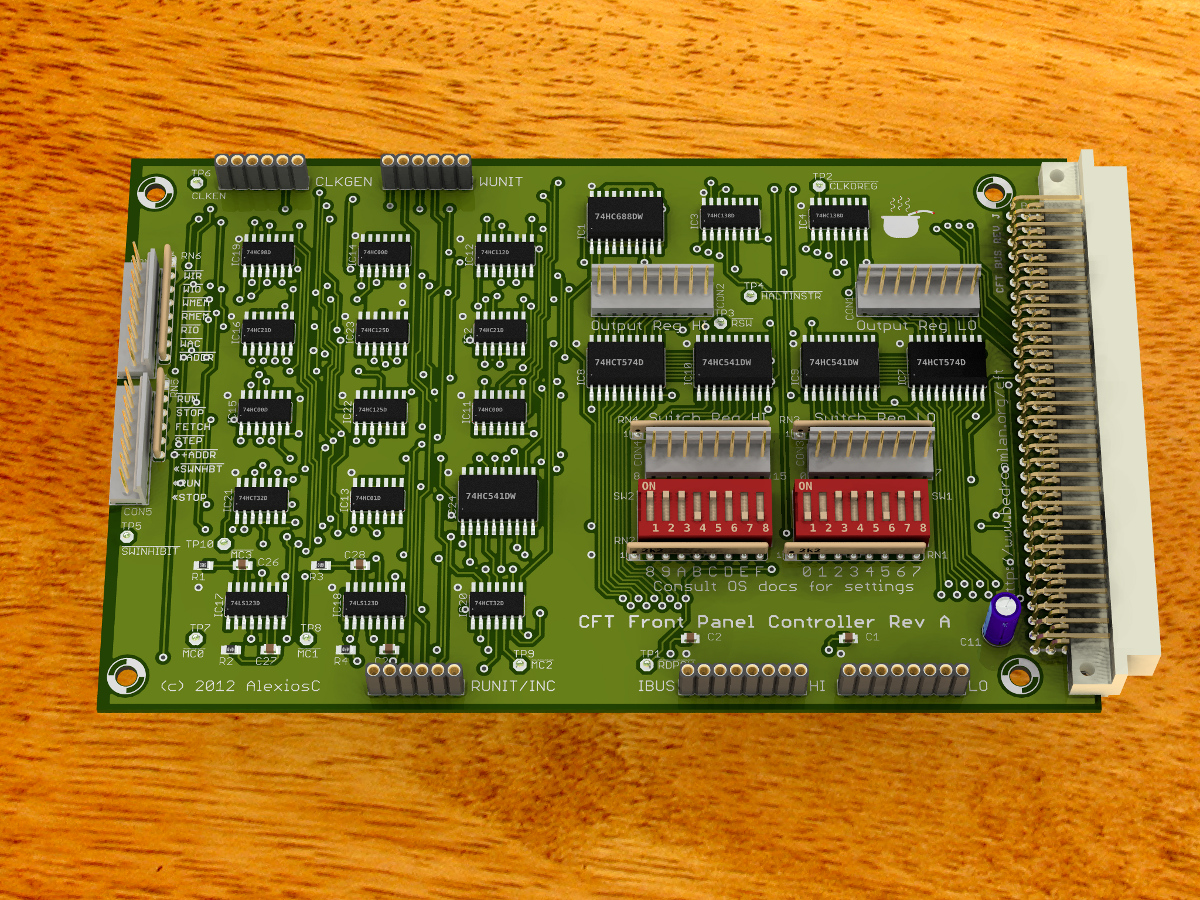
\includegraphics[width=0.8\textwidth]{figs/front-panel-controller-smd.jpg}\\
\caption{\label{fig-rendered-fpc-smd}Rendered view of the \abbr{SMD} revision of the
  Front Panel Controller board.}
\end{figure*}


The Front Panel comprises three distinct parts (though parts 2 and 3
may be implemented on the same physical board):

\begin{enumerate}
\item{\bfseries The Front Panel Controller Card} contains most of the front
  panel logic.
\item{\bfseries The Front Panel Driver and LED Board} hosts the LEDs and
  their drivers, as well as the Multi-Function display logic. The LED
  banks are connected directly to the corresponding processor hardware
  (e.g. the register card) using 8 or 9-conductor flat cables.
\item{\bfseries The Front Panel Debounce and Switch Board} hosts the switches
  and their debounce circuitry.
\end{enumerate}

\subsection{Connectors}

The Front Panel Controller Card connects to the switch and LED boards
via six 8-conductor cables.

\begin{table}[tb]
  \caption{\label{tab-connectors}Connections between the front panel
    and the processor.}
  \footnotesize
  \centering
  \zebra
  \begin{tabular}{llcll}
    \noalign{\smallskip}\hline\noalign{\smallskip}
    Function & Name & Conductors & From & To \\
    \noalign{\smallskip}\hline\noalign{\smallskip}
    Switch Register Low      & CON1  & 8 & Switch board & Front Panel Controller \\
    Switch Register High     & CON2  & 8 & Switch board & Front Panel Controller \\
    Memory Banking Status    & CON3  & 9 & Memory Banking board & Front Panel LED board \\
    \A{} Low                 & CON4  & 8 & Register or ALU board & Front Panel LED board \\
    \A{} High                & CON5  & 8 & Register or ALU board & Front Panel LED board \\
    \PC{} Low                & CON6  & 8 & Register board & Front Panel LED board \\
    \PC{} High               & CON7  & 8 & Register board & Front Panel LED board \\
    \IR{} Low                & CON8  & 8 & Control board & Front Panel LED board \\
    \IR{} High               & CON9  & 8 & Control board & Front Panel LED board \\
    Microcode Vector Low     & CON10 & 8 & Control board & Front Panel LED board \\
    Microcode Vector Medium  & CON11 & 8 & Control board & Front Panel LED board \\
    Microcode Vector High    & CON12 & 8 & Control board & Front Panel LED board \\
    Flags                    & CON13 & 5 & Control board \& ALU & Front Panel LED board \\
    Output Register Low      & CON14 & 8 & Front Panel Controller & Front Panel LED board \\
    Output Register High     & CON15 & 8 & Front Panel Controller & Front Panel LED board \\
    \DR{} Low                & CON16 & 8 & Register board & Front Panel LED board \\
    \DR{} High               & CON17 & 8 & Register board & Front Panel LED board \\
    Microcode Address Low    & CON18 & 8 & Control board & Front Panel LED board \\
    Microcode Address High   & CON19 & 7 & Control board & Front Panel LED board \\
    Interrupt Flag Status    & CON20 & 8 & Interrupt Controller board & Front Panel LED board \\
    Interrupt Enable Status  & CON21 & 8 & Interrupt Controller board & Front Panel LED board \\
    Control switches 1       & CON22 & 8 & Switch board & Front Panel Controller \\
    Control switches 2       & CON23 & 8 & Switch board & Front Panel Controller \\
    Miscellaneous signals    & CON24 & 9 & Switch board & (various cards) \\
    Miscellaneous LEDs (×3)  & SV1   & 6 & Any required & Front Panel LED board \\
    \noalign{\smallskip}\hline\noalign{\smallskip}
  \end{tabular}
\end{table}

\subsection{Front Panel Configuration}

The front panel is configurable using jumpers and trimmers.

\subsubsection{\sw{STEP} Autorepeat Tuning}

The autorepeat delay and repeat rate may be modified by varying the
trimmers \schpt{R1} (autorepeat delay) and \schpt{R4} (repeat
rate). Please ensure that the autorepeat rate is not faster than the
slowest CPU clock, otherwise the instruction stepping mechanism will
break.

\subsubsection{Fetch/Execute Decoder}

The fetch/execute decoder is used to control the \lt{FETCH} and
\lt{EXEC}. It also provides input to the Front Panel Controller so
that instruction stepping stops immediately after a fetch cycle. Fetch
decoding compares the least significant bits of the 4-bit μPC register
(the high order bit is assumed to be 0, since no microcode ROM is
expected to have an 8-step fetch cycle). The \abbr{DIP} switch block
\schpt{SW1} encodes (in binary) the value of the μPC for the first
step of the {\em Execute\/} cycle. For Microcodes up to version 3,
this value is 3 (\bin{011}).

\subsubsection{Light Control Jumpers}

A number of three-pin jumpers on the front panel control the behaviour
of many banks of console lights depending on the position of the
\sw{VERBOSE}/\sw{TERSE} switch. A jumper shunt may be placed across
pins 1–2 to leave a bank on regardless of the setting of the switch,
or across pins 2–3 to allow the bank to be turned off when the
\sw{VERBOSE}/\sw{TERSE} switch is in the \sw{TERSE} position.

If non-CMOS technology is used for the front panel LED buffers (e.g. 74LS541N
instead of 74HC541N), removing the jumper shunt altogether disables the light
bank. \caution{This setting can cause erratic behaviour and/or damage to CMOS
  light buffers.}

This is a list of light control jumpers:

\begin{description}
\item{\schpt{JP1}} — the Memory Banking display. 
\item{\schpt{JP2}} — the Instruction Register display.
\item{\schpt{JP3}} — the Microcode Vector display.
\item{\schpt{JP4}} — the Flag display.
\item{\schpt{JP5}} — the Interrupt Status display.
\end{description}

\subsection{Connections}

The front panel boards connect to the processor by means of numerous
8-way connectors, shown in~\tcf{tab-connectors}.


\section{Theory of Operation}

The front panel is an unexpectedly complex device with a number of
interwoven parts, and merits some description.

\subsection{Switches}

In their most general form, front panel switches connect between ground and the
input pin of a CMOS device. When switches are closed, they provide a logic 0 to
the attached circuitry. When they are opened, they float — this necessitates a
pull-up resistor for each switch to provide a logic 1. The pull-ups are placed
nearest the IC inputs, especially in cases where the switches are connected via
connectors that may malfunction or break.

\subsection{Switch Lock-Out}

Many switches can be secured against accidental or malicious operation. There
are two mechanisms to provide this feature:

\begin{itemize}
  \item The \ns{LOCK} signal. This is at +0V when the panel is unlocked, and a
    high-impedance line when the panel is locked.  The panel key switch
    physically connects the \ns{LOCK} signal to ground when the panel is
    unlocked, so the fan-out of this signal is not an issue.  Switches
    connecting to this signal rather than ground will only register when the
    \ns{LOCK} is at ground level, which will only happen when the key lock is
    in the \sw{PANEL} position.  This is used by the asynchronous action
    switches in the system, namely \sw{RUN}, \sw{STOP}, \sw{IFR1} and
    \sw{IFR6}.

  \item The \ns{SAFE} signal. This is generated by an open-drain NAND gate
    which combines the \ns{SWINHIBIT} and \ns{LOCK} signals. \ns{SWINHIBIT} is
    an input from the Front Panel Controller card, and is low when the system
    is running. When either \ns{SWINHIBIT} or \ns{LOCK} are low, the open drain
    NAND gate is in the high-Z state, effectively disconnecting \ns{SAFE} and
    rendering useless those switches that use it. When both \ns{SWINHIBIT} and
    \ns{LOCK} are high (inactive), the open drain NAND gate sinks current, and
    any switches using \ns{SAFE} can be operated. This is used for switches
    that should have no effect while the system is running, or the panel is
    locked.
\end{itemize}

Please consult~\tcf{tab-swlockout} for a listing of front panel switches and
how they are locked out.

\subsection{Switch Debouncing}

Switches are debounced using the fairly standard circuit illustrated
in~\fcf{fig-switch-debounce}. The passive components smooth the effect of the
switch bouncing and provide a fairly sluggish ramp up (or down). The Schmitt
trigger inverter converts this to the appropriate logic value. The values of
the resistors and capacitor may be changed to accommodate various types of
switch pathology. This debouncer is purposefully slow, since the front panel is
not meant to have sub-millisecond responses.

\begin{figure}
\centering
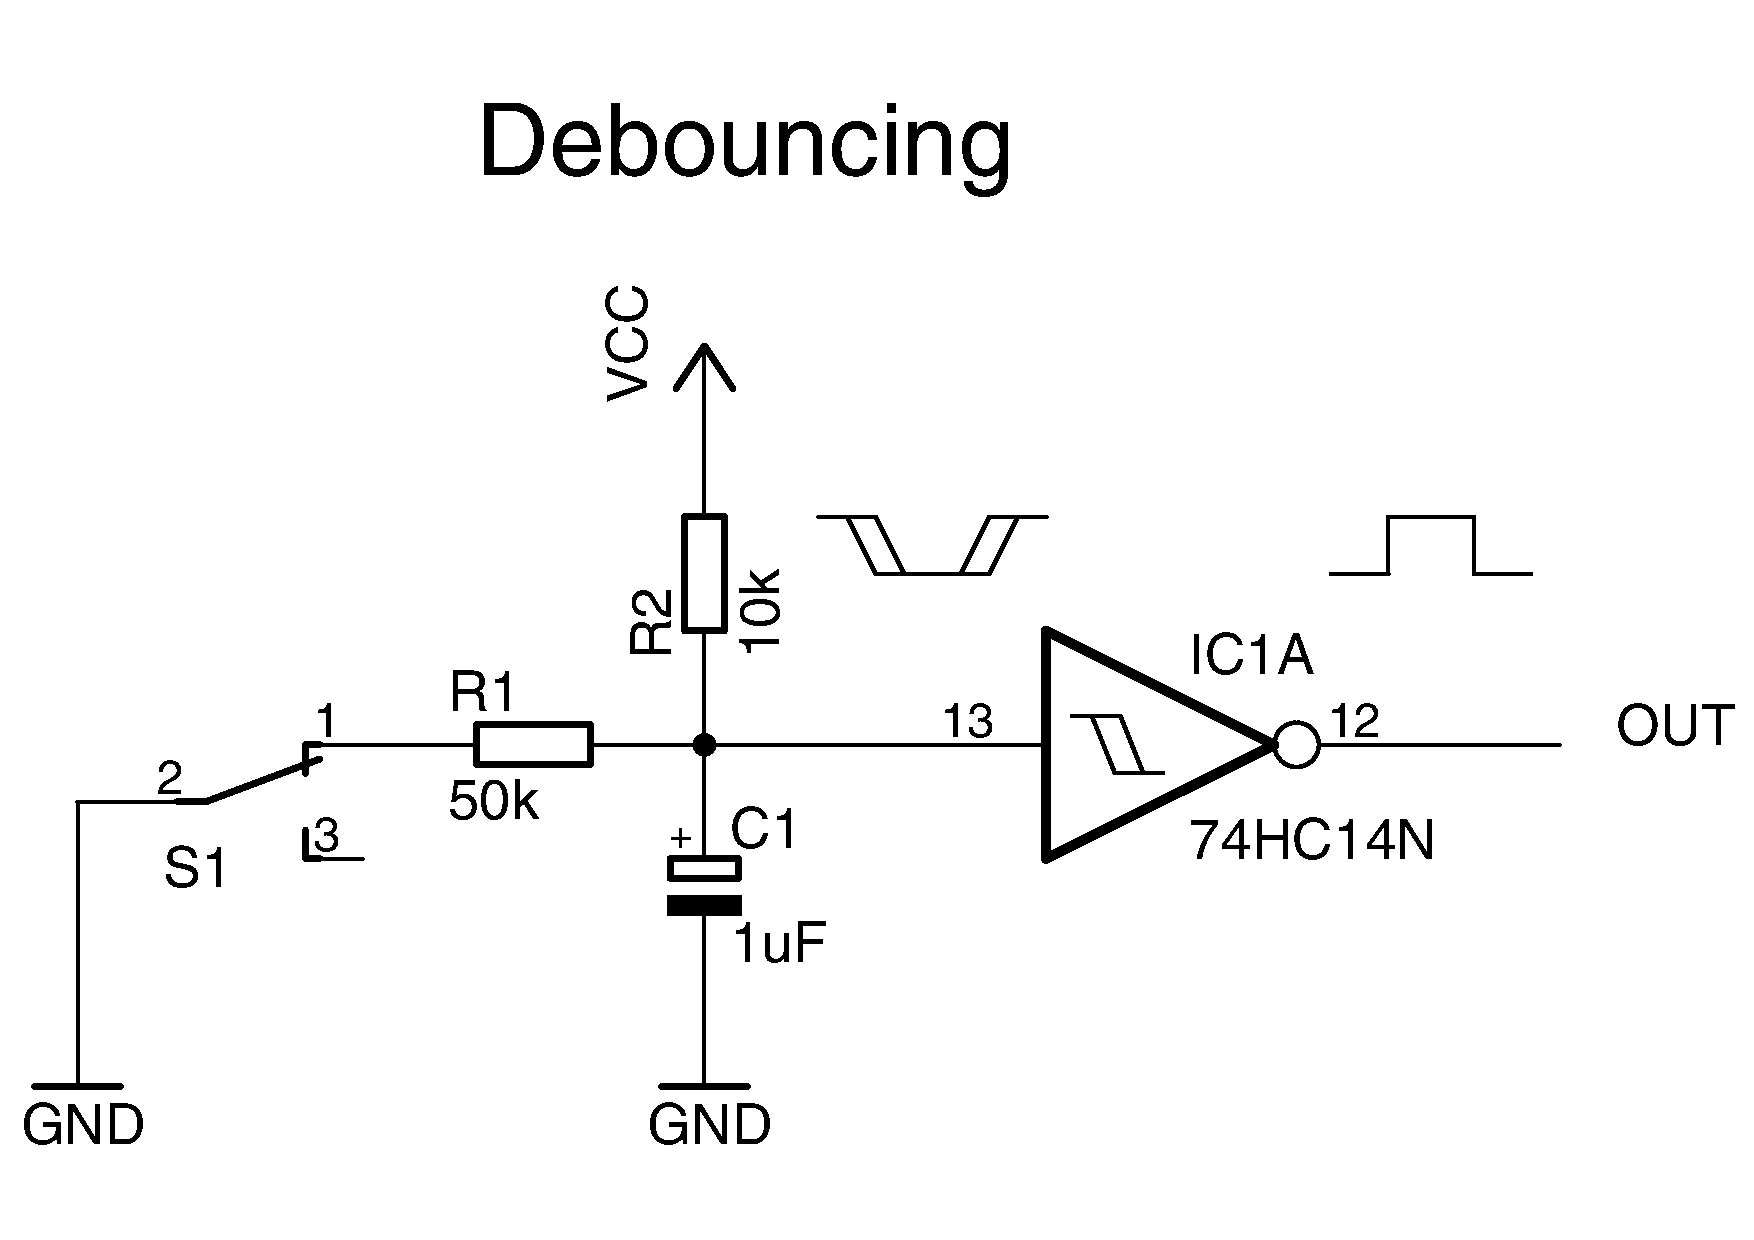
\includegraphics[width=0.85\columnwidth]{figs/debouncing.pdf}\\
\caption{\label{fig-switch-debounce}Switch debouncing.}
\end{figure}

\begin{table}[tb]
  \footnotesize
  \caption[Front Panel switch lock-out]{\label{tab-swlockout}Switch lock-out. Switches locked out with
    \ns{SAFE} are enabled with the panel unlocked and the processor
    stopped. Switches locked out with \ns{LOCK} are enable with the panel
    unlocked.}  \centering
  \zebra
  \begin{tabular}{lp{0.4\textwidth}p{0.3\textwidth}}
    \noalign{\smallskip}\hline\noalign{\smallskip}
    Switch & Function & Lock out \\
    \noalign{\smallskip}\hline\noalign{\smallskip}
    \schpt{S1–S16} & Switch Register bits 0–15 & Not locked out. Read by software or actuation of other switches) \\
    \schpt{S17} & Key switch & Not locked out. Provides lock-out mechanism to other switches. \\
    \schpt{S18} & \sw{VERBOSE}\ /\ \sw{TERSE}       & Not locked out, only modifies front panel output.\\
    \schpt{S19} & \sw{ROM HI}\ /\ \sw{RAM HI}       & \ns{SAFE}.\\
    \schpt{S20} & \sw{FAST}\ /\ \sw{SLOW}\ /\ \sw{TEST} & \ns{SAFE}.\\
    \schpt{S21} & \sw{uSTEP}\ /\ \sw{STEP}          & \ns{SAFE}.\\
    \schpt{S22} & \sw{START}\ /\ \sw{RESET}         & \ns{LOCK}.\\
    \schpt{S23} & \sw{LOAD ADDR}                & \ns{SAFE}.\\
    \schpt{S24} & \sw{LOAD IR}\ /\ \sw{LOAD AC}      & \ns{SAFE}.\\
    \schpt{S25} & \sw{MEMORY DEPOSIT}\ /\ \sw{MEMORY DEP NEXT} & \ns{SAFE}.\\
    \schpt{S26} & \sw{MEMORY EXAMINE}\ /\ \sw{MEMORY EXAM NEXT} & \ns{SAFE}.\\
    \schpt{S27} & \sw{I/O DEPOSIT}\ /\ \sw{I/O DEP NEXT} & \ns{SAFE}.\\
    \schpt{S28} & \sw{I/O EXAMINE}\ /\ \sw{I/O EXAM NEXT} & \ns{SAFE}.\\
    \schpt{S29} & \sw{OUTPUT REG}\ /\ \sw{DR}\ /\ \sw{uADDR VEC} & Not locked out, only modifies front panel output.\\
    \schpt{S30} & \sw{RUN}\ /\ \sw{STOP}            & \ns{LOCK}.\\
    \schpt{S31} & \sw{IFR6}\ /\ \sw{IFR1}           & \ns{LOCK}.\\
    \noalign{\smallskip}\hline\noalign{\smallskip}
  \end{tabular}
\end{table}


\subsection{Sequencing}

A simple sequencer based on two dual 74LS123 multivibrator chips is used to
provide timing for the front panel's memory and I/O functionality. The
waveforms are neither as accurate nor as fast as the ones generated by the
control unit itself, but the front panel is a human interface device, so this
is not a requirement. The waveforms {\em are\/} properly interlocked to allow
read and write access to memory and I/O-space locations. 

The sequencer starts when any of the ‘exam’ or ‘deposit’ switches are actuated,
in either the normal or increment (‘next’) position. This includes eight
functions: \sw{MEMORY DEPOSIT}, \sw{MEMORY DEP NEXT}, \sw{MEMORY EXAMINE},
\sw{MEMORY EXAM NEXT}, \sw{INPUT/OUTPUT DEPOSIT}, \sw {INPUT/OUTPUT DEP NEXT},
\sw{INPUT/OUTPUT EXAMINE} and \sw{INPUT/OUTPUT EXAM NEXT}.

\begin{table}[tb]
  \caption[Internal wiring of the Memory and I/O switches]{\label{tab-fpcycles}The internal wiring of the eight memory and I/O
    switches (provided by four physical momentary switches with momentary up
    and down positions).}  \centering
  \footnotesize
  \zebra
  \begin{tabular}{lccccc}
    \noalign{\smallskip}\hline\noalign{\smallskip}
    Switch & \ns{FPWMEM} & \ns{FPRMEM} & \ns{FPWIO} & \ns{FPRIO} & \ns{FPINCADDR} \\
    \noalign{\smallskip}\hline\noalign{\smallskip}
    \sw{MEMORY DEPOSIT} & Assert & & & & \\
    \sw{MEMORY DEP NEXT} & Assert & & & & Assert \\
    \sw{MEMORY EXAMINE} & & Assert & & & \\
    \sw{MEMORY EXAM NEXT} & & Assert & & & Assert \\
    \sw{INPUT/OUTPUT DEPOSIT} & & & Assert & & \\
    \sw{INPUT/OUTPUT DEP NEXT} & & & Assert & & Assert \\
    \sw{INPUT/OUTPUT EXAMINE} & & & & Assert & \\
    \sw{INPUT/OUTPUT EXAM NEXT} & & & & Assert & Assert \\
    \noalign{\smallskip}\hline\noalign{\smallskip}
  \end{tabular}
\end{table}


Depending on whether it was a \sw{MEMORY} or \sw{INPUT/OUTPUT} switch, whether
it was a \sw{EXAMINE} (read) or \sw{DEPOSIT} (write) switch, and whether or not
the \sw{NEXT} (increment address) function was selected, the sequencer connects
its four outputs to appropriate bus lines to perform the requested cycle. 

consists of a tri-state buffer and
a pull-up resistor. The buffer's enable line is connected to the \ps{RUN}
signal. When the processor is running, the buffer tri-states its output. The
pull-up resistor ensures

The raw sequencer outputs are shown in~\fcf{fig-panel-mc}. Please note that, in
order to show the relationships of the timing rather than the widths of the
pulses, the waveforms are not to scale.

The sequencer starts on the falling edge of \ns{MCSTART}, obtained by ANDing
the front panel signals \ns{FPWMEM}, \ns{FPRMEM}, \ns{FPWIO} and \ns{FPRIO}.

Signals \ns{MC0} and \ns{MC1} are synchronised with the falling edge of
\ns{MCSTART}. Signals \ns{MC2} and \ns{MC3} are synchronised with the rising
edge of \ns{MC1}. This forms two separate sub-cycles in the waveform. The first
sub-cycle is used to load the \MAR{} register with the current address stored
in the \PC{} register. The second sub-cycle is responsible for the memory or
I/O operation, and is also responsible for incrementing \PC{} if the
\ns{FPINCADDR} signal has been asserted.

When the sequencer is idle, all of its outputs are tri-stated to avoid
contending with the control unit. The sequencer must not be started with the
processor operating. To avoid this, a safety interlock is in place. The buffer
lies between the output of the And gate and the \ps{MCSTART} signal. With the
buffer tri-stated, the pull-up resistor pulls \ps{MCSTART} high, disabling the
sequencer. When the buffer is enabled, the And gate is allowed to drive
\ps{MCSTART} low, starting the sequencer.

Please refer to~\fcf{fig-panel-mcw} for the write cycle waveform
and~\fcf{fig-panel-mcr} for the read cycle waveform. Both apply to memory and
I/O operations. \ns{INCPC} is only strobed if the respective switch was
operated in the ‘next’ position, i.e.\ \ns{FPINCADDR} strobed. Control signals
are tri-stated when \ns{MCSTART} is high, which implies that the front panel
switch must be held active by the operator until the end of the cycle. This is
not expected to be a problem, as the entire cycle typically lasts approximately
180–900~ns.

\subsubsection{Wait States and the Front Panel}

For simplicity, the front panel's sequencer ignores the \ns{WS} signal
entirely. Memory and I/O cycles cannot be prolonged
externally. However, since the front panel is operated by humans, its
memory and I/O cycles have a period in the order of milliseconds,
three orders of magnitude slower than the processor's otherwise
equivalent cycles. This accommodates even the slowest devices.

There may be exotic exceptions and subtle ways of abusing the
\gls{Wait State} mechanism which the front panel fails to activate or
take advantage of. This is a limitation of the design, but it keeps
the chip count low.

\subsubsection{Sequencer Glitch}

Due to the design of the sequencer, a cycle will be {\em aborted\/}
should the actuating switch be released during the course of the
cycle. This is an unlikely occurrence, since the cycle period is in
the order of milliseconds, but is worth noting.

\begin{figure}[tb]
\centering
\begin{tikztimingtable}
  %\ns{MCSTART} & 2H h e N(A0) 10L 11e H h \\
  \ns{MCSTART} & 2H h e N(A0) 15L s l s l \\
  \ns{MC0}     & 3H     N(A1) 4L  13H \\
  \ns{MC1}     & 3H     N(A2) 6L  N(B2) 11H \\
  \ns{MC2}     & 9H               N(B3) 8L 3H \\
  \ps{MC3}     & 9H               N(B4) 5L 6H \\
\extracode
  \tablerules
  \begin{pgfonlayer}{background}
    \draw [help lines] (A0) -- (A2);
    \draw [help lines] (B2) -- (B4);
  \end{pgfonlayer}
\end{tikztimingtable}
\caption[Waveforms generated by the front panel
  sequencer]{\label{fig-panel-mc}Waveforms generated by the front panel
  sequencer. The front panel controller connects these waveforms to different
  control unit signals to allow read and write access to memory and I/O space
  locations.}
\end{figure}

\begin{figure}[t]
\centering
\begin{tikztimingtable}
  \ns{MCSTART}                & 2H h N(A0)     15L l           N(D0)   2H \\
  \ns{WAR}                    & 2Z z   N(A1)     3L  12H               h 2Z \\
  \ns{RPC}                    & 2Z z             5L  N(B2) 10H         h 2Z  \\
  \ns{MEM}/\ns{IO}            & 2Z z         5H      7L 3H             h 2Z  \\
  \ns{INCPC}                  & 2Z z         5H      7L 3H             h 2Z  \\
  \ns{R}                      & 2Z z         5H      7L 3H             h 2Z  \\
  \ns{WAC}                    & 2Z z   N(A2) 5H      N(B4) 4L 6H h N(D2) 2Z \\
\extracode
  \tablerules
  \begin{pgfonlayer}{background}
    \draw [help lines] (A0) -- (A2);
    \draw [help lines] (B2) -- (B4);
    \draw [help lines] (D0) -- (D2);
  \end{pgfonlayer}
\end{tikztimingtable}
\caption[Memory (or I/O) read cycle]{\label{fig-panel-mcr}
  Memory (or I/O) read cycle. \ns{INCPC} is only
  strobed if \ns{FPINCADDR} has been asserted.}
\end{figure}

\begin{figure}[t]
\centering
\begin{tikztimingtable}
  \ns{MCSTART}                & 2H h N(A0)     15L l           N(D0)   2H \\
  \ns{WAR}                    & 2Z z   N(A1)     3L  12H               h 2Z \\
  \ns{RPC}                    & 2Z z             5L  N(B2) 10H         h 2Z  \\
  \ns{MEM}/\ns{IO}            & 2Z z         5H      7L 3H             h 2Z  \\
  \ns{INCPC}                  & 2Z z         5H      7L 3H             h 2Z  \\
  \ns{RAC}                    & 2Z z         5H      7L 3H             h 2Z  \\
  \ns{W}                      & 2Z z   N(A2) 5H      N(B4) 4L 6H h N(D2) 2Z \\
\extracode
  \tablerules
  \begin{pgfonlayer}{background}
    \draw [help lines] (A0) -- (A2);
    \draw [help lines] (B2) -- (B4);
    \draw [help lines] (D0) -- (D2);
  \end{pgfonlayer}
\end{tikztimingtable}
\caption[Memory (or I/O) write cycle]{\label{fig-panel-mcw} Memory (or
  I/O) write cycle. \ns{INCPC} is only strobed if \ns{FPINCADDR} has
  been asserted.}
\end{figure}

\subsection{The Front Panel System Device}

The front panel contains a System Device: hardware attached to the computer's
expansion bus and addressable by the processor by means of I/O
operations. System devices occupy I/O space addresses between
\hex{0000}–\hex{00FF} (inclusive). The processor provides the convenient signal \ns{SYSDEV}
on the bus, driven low when I/O addresses in this range are selected.

The Front Panel Controller uses this to decode I/O space addresses
\hex{0008}-\hex{000F} using a 74x688 comparator and two 74x138 demultiplexers
(one for reading, one for writing). Of the total sixteen control lines, four
are used to provide the following four CFT I/O addresses:

%% \extcmd{SR0}{IN R \&8}{4408}{-r-vehf}{008}%
%%        {PFP, Read Switch Register}%
%%        {%
%%          Reads 16 bits from the front panel Switch Register into the
%%          \gls{Accumulator}. This allows a program to read input from the panel operator.

%%          Verilog support for this is rudimentary.
%%        }

\extcmd{SR1}{IN R \&9}{4409}{-r-vehf}{009}%
       {PFP, Read DIP Switch Register}%
       {%
         Reads 16 bits from the Front Panel Controller DIP
         switches. This is used to provide a set of ‘turn-key’
         settings to the operating system, such as the address of a
         boot block, the base address of a console, serial parameters,
         et cetera. The semantics of the DIP switches have not yet
         been decided on. Two or three of them may be hard-wired to
         allow autodetection of the CFT platform (Verilog, Emulation
         or Hardware).

         Verilog support for this is rudimentary.
       }

\extcmd{FPOR}{OUT R \&a}{540a}{-r-vehf}{00a}%
       {PFP, Write Front Panel Output Register}%
       {%
         Writes 16 bits from the \gls{Accumulator} to the front panel
         Output Register. This may be used to output data to the panel operator.

         Verilog support for this is rudimentary.
       }

\extcmd{HALT}{OUT R \&a}{540a}{c-wvehf}{00a}%
       {PFP, Halt Processor}%
       {%
         Stops the computer, simulating the actuation of the front
         panel \sw{STOP} switch. The computer can only be resumed from
         the front panel.
       }

Most normal peripherals attach themselves to the Address Bus and Data Bus,
relying on the processor to connect the latter to the \IBUS{} when a memory or
I/O operation is taking place. The Front Panel System Device attaches to the
Address Bus and {\em \IBUS{}\/} instead. \caution{Note: this is a bug. It must
  be fixed, or bus contention may occur.}

\section{Front Panel Assembly Construction}

The following sections contain bills of materials, part indexes and schematics
for the Front Panel Assembly which contains the lights and switches of the
front panel.




%% \subsection{Bill of Materials}

%% This section provides a bill of materials for the front panel assembly. This
%% is meant for personal reference, and is not exhaustive by any means.

%% This project is not endorsed, funded or supported by Farnell or RS Components
%% in any way.

%% \bomv{front-panel}

%% \subsection{Part Index}

%% This section provides an index of parts used on the front panel. It is
%% provided for reference only, and is not necessarily correct.

%% This project is not endorsed, funded or supported by Farnell or RS Components
%% in any way.

%% \bomp{front-panel}

%
% Controller
%

\section{Front Panel Controller}

The following sections contain bills of materials, part indexes and schematics
for the Front Panel Controller board which interfaces the Front Panel Assembly
to the processor and computer at large.

%% \subsection{Bill of Materials}

%% This section provides a bill of materials for the front panel controller. This
%% is meant for personal reference, and is not exhaustive by any means.

%% This project is not endorsed, funded or supported by Farnell or RS Components
%% in any way.

%% \bomv{front-panel-controller}

%% \subsection{Part Index}

%% This section provides an index of parts used on the front panel controller. It is
%% provided for reference only, and is not necessarily correct.

%% This project is not endorsed, funded or supported by Farnell or RS Components
%% in any way.

%% \bomp{front-panel-controller}

%%  LocalWords:  documentclass CFT Alexios PDP autoindexing Von LSI Chouchoulas
%%  LocalWords:  Neumann microprograms microprogram microinstructions Bauform
%%  LocalWords:  et cetera kiloword KWord kilowords KWords Autoindex rp GND CLC
%%  LocalWords:  SUBRET JSR TRAPRET ISRRET ISR autoindex th FC FFF tl RSTIN tri
%%  LocalWords:  FFFF pagerel vlgrey linewidth fillstyle fillcolor de GPULSE lp
%%  LocalWords:  addr FFFE IOT LIA JMP bitwise ORred asm bitfield CLA DMA IRQ
%%  LocalWords:  CLL RBL RBR RNL RNR NOP linearc SNA SZA SSL SNN SNZ LEDs
%%  LocalWords:  SCL CLI STI SNP lll RET RTT SBL SBR SNL SNR TTY AEXT Debounce
%%  LocalWords:  disjuncted conjuncted ANDed MWord MEM uSTEP DEP BNK Autorepeat
%%  LocalWords:  microinstruction kWords IFR uADDR VEC kWord llcll SV SWINHIBIT
%%  LocalWords:  ALU Microcodes CMOS HC Farnell swlockout Debouncing
